\let\lesson\undefined
\newcommand{\lesson}{\phantomlesson{Bài 16.}}
\setcounter{section}{2}
\section{Trắc nghiệm}
\ANSMCQ
{	\begin{center}
		\begin{tabular}{|m{2.8em}|m{2.8em}|m{2.8em}|m{2.8em}|m{2.8em}|m{2.8em}|m{2.8em}|m{2.8em}|m{2.8em}|m{2.8em}|}
			\hline
			1.D  & 2.D  & 3.D  & 4.B  & 5.B  &   &   &   &   &   \\
			\hline
		\end{tabular}
	\end{center}
}
\begin{enumerate}[label=\bfseries Câu \arabic*:, leftmargin=1.5cm]
	\item \mkstar{1}\\
	Phát biểu nào sau đây là \textbf{không đúng} khi nói về hiệu suất?
	\begin{mcq}
		\item Hiệu suất của động cơ luôn nhỏ hơn 1.
		\item Hiệu suất đặc trưng cho mức độ hiệu quả của động cơ.
		\item Hiệu suất của động cơ được xác định bằng tỉ số giữa công suất có ích và công suất toàn phần.
		\item Hiệu suất được xác định bằng tỉ số giữa năng lượng đầu ra và năng lượng đầu vào.
	\end{mcq}
\hideall{
\textbf{Đáp án D.}\\
Hiệu suất được xác định bằng tỉ số giữa năng lượng đầu ra và năng lượng đầu vào.
}

\item \mkstar{1}\\
Hiệu suất càng cao thì
\begin{mcq}
	\item tỉ lệ năng lượng hao phí so với năng lượng toàn phần càng lớn
	\item năng lượng tiêu thụ càng lớn.
	\item năng lượng hao phí càng ít.
	\item tỉ lệ năng lượng hao phí so với năng lượng toàn phần càng ít.
\end{mcq}
\hideall{
\textbf{Đáp án D.}
}

\item \mkstar{2}\\
Hiệu suất của một quá trình chuyển hóa công được kí hiệu là $H$. Vậy $H$ luôn có giá trị
\begin{mcq}(4)
	\item $H>1$.
	\item $H=1$.
	\item $H<1$.
	\item $0<H\le 1$.
\end{mcq}
\hideall{
\textbf{Đáp án D.}
}

\item \mkstar{2}\\
{Một động cơ có công suất tiêu thụ bằng $\SI{5}{\kilo\watt}$ kéo một vật có trọng lượng $\SI{12}{\kilo\newton}$ lên cao $\SI{30}{\meter}$ theo phương thẳng đứng trong thời gian $\SI{90}{\second}$ với vận tốc không đổi. Hiệu suất của động cơ bằng
\begin{mcq}(4)
	\item $\SI{100}{\percent}$.
	\item $\SI{80}{\percent}$.
	\item $\SI{60}{\percent}$.
	\item $\SI{40}{\percent}$.
\end{mcq}
}
\hideall{
\textbf{Đáp án B.}\\
Công cần thiết để kéo vật nặng lên cao $\SI{30}{\meter}$:
$$A_i=Ph=\SI{360}{\kilo\joule}$$
Công suất có ích để kéo vật:
$$\calP_i=\dfrac{A_i}{t}=\SI{40}{\kilo\watt}$$
Hiệu suất động cơ:
$$H=\dfrac{\calP_i}{\calP_{tp}}\cdot\SI{100}{\percent}=\SI{80}{\percent}.$$
}

\item \mkstar{3}\\
{Một máy bơm nước mỗi giây có thể bơm được 15 lít nước lên bể ở độ cao $\SI{10}{\meter}$. Hiệu suất của máy bơm là 0,7. Lấy $g=\SI{10}{\meter/\second^2}$. Biết khối lượng riêng của nước là  $D=\SI{E3}{\kilogram/\meter^3}$. Sau nửa giờ máy bơm đã thực hiện một công bằng
	\begin{mcq}(4)
		\item $\SI{1500}{\kilo\joule}$.
		\item $\SI{3857}{\kilo\joule}$.
		\item $\SI{1890}{\kilo\joule}$.
		\item $\SI{7714}{\kilo\joule}$.
	\end{mcq}

}
\hideall{
\textbf{Đáp án B.}\\
Khối lượng nước được bơm lên sau nửa giờ:
$$m=D\cdot V=\left(\SI{1000}{\kilogram/\meter^3}\right)\cdot\left(\SI{15E-3}{\meter^3}\right)\cdot\left(\SI{1800}{\second}\right)=\SI{27E3}{\kilogram}$$
Công có ích máy bơm cần thực hiện để bơm lượng nước trên lên cao $\SI{10}{\meter}$:
$$A_i=mgh=\SI{2700}{\kilo\joule}$$
Công toàn phần máy bơm thực hiện:
$$A_\text{tp}=\dfrac{A_i}{H}=\SI{3857}{\kilo\joule}.$$
}

\end{enumerate}

\section{Tự luận}
\begin{enumerate}[label=\bfseries Câu \arabic*:, leftmargin=1.5cm]
	\item \mkstar{2}
	
	
	{
		Em hãy chỉ ra những loại năng lượng cần cung cấp để động cơ xe máy hoặc xe ô tô vận hành. Thảo luận những yếu tố ảnh hưởng đến hiệu suất của động cơ xe.
	}
	
	\hideall
	{	
		Những loại năng lượng cần cung cấp để động cơ xe máy hoặc xe ô tô vận hành: hóa năng, nhiệt năng, động năng, điện năng,..vv 
		
		Những yếu tố dảnh hưởng đến hiệu suất của động cơ xe là: lực ma sát và các dạng năng lượng hao phí khác.
	}
	\item \mkstar{2}
	
	
	{
		Em hãy đề xuất giải pháp làm tăng hiệu suất của quạt điện sau một thời gian sử dụng. Giải thích lí do lựa chọn giải pháp này.
	}
	
	\hideall
	{	
		Giải pháp làm tăng hiệu suất của quạt điện sau một thời gian sử dụng: Lau bớt bụi bẩn bám trên cánh quạt và lồng quạt, tra thêm dầu mỡ vào bộ phận quay của quạt.
		
		Giải thích:
		
		+ Lau bụi bẩn để làm giảm ma sát giữa cánh quạt với không khí và để gió thoát ra được nhiều hơn.
		
		+ Tra thêm dầu mỡ để giảm ma sát giữa bộ phận đứng yên và bộ phận quay. 
	}

	
	\item \mkstar{3}
	
	
	{
		Một ô tô chuyển động với vận tốc $\SI{54}{km/h}$ có thể đi được đoạn đường dài bao nhiêu khi tiêu thụ hết 60 lít xăng? Biết động cơ của ô tô có công suất $\SI{45}{kW}$; hiệu suất $25\%$; $\SI{1}{kg}$ xăng đốt cháy hoàn toàn tỏa ra nhiệt lượng bằng $\xsi{46\cdot 10^6}{J/kg}$ và khối lượng riêng của xăng là $\SI{700}{kg/m^3}$.
	}
	
	\hideall
	{	
		Đổi $\SI{54}{km/h} = \SI{15}{m/s}; \SI{45}{kW} = \SI{45000}{W}.$
		
		Gọi $s$ là quãng đường đi được khi động cơ tiêu thụ hết 60 lít xăng.
		
		Khối lượng 60 lít xăng:
		
		$$m = DV = \SI{42}{kg}.$$
		
		Công thực hiện của động cơ:
		
		$$A = \calP t = \calP \dfrac{s}{v}.$$
		
		Nhiệt lượng do 60 lít xăng khi bị đốt cháy hoàn toàn tỏa ra là 
		
		$$Q = qm.$$
		
		Ta có:
		
		$$H = \dfrac{A}{Q} \Rightarrow A = HQ  \Leftrightarrow P \dfrac{s}{v} = Hqm \Rightarrow s = \SI{161000}{m} = \SI{161}{km}.$$
		
		Vậy khi tiêu thụ hết 60 lít xăng, ô tô có thể đi được quãng đường là $\SI{161}{km}.$
	}
	\item \mkstar{2}
	
	
	{
		Máy tời đang hoạt động với công suất $\SI{1000}{W}$ đưa $\SI{100}{kg}$ vật liệu lên đều tới độ cao $\SI{16}{m}$ trong $\SI{20}{s}$. Tính hiệu suất của máy tời.
	}
	
	\hideall
	{	
		Năng lượng có ích:
		
		$$W_\text{ci} = mgh = \SI{16000}{J}.$$
		
		Năng lượng toàn phần của máy
		
		$$W = A = Pt = \SI{20000}{J}.$$
		
		Hiệu suất của máy tời là:
		
		$$H =\dfrac{W_\text{ci}}{W} = 80\%.$$
	}
	
	

	\item \mkstar{2}
	
	
	{
		Khi đưa một vật lên cao $\SI{2,5}{m}$ bằng mặt phẳng nghiêng, người ta phải thực hiện một công là $\SI{3600}{J}$. Biết hiệu suất của mặt phẳng nghiêng là $75\%$. Tính khối lượng của vật đó. Lấy $g = \SI{10}{m/s}^2$.
	}
	
	\hideall
	{	Ta có:
		
		$$H = \dfrac{W_\text{ci}}{W} = \dfrac{Ph}{A}.$$
		
		Trọng lượng của vật
		
		$$P = \dfrac{HA}{h} = \SI{1080}{N}.$$
		
		Khối lượng của vật đó
		
		$$m = \dfrac{P}{g} = \SI{10,8}{kg}.$$
	}
	\item \mkstar{2}
	
	
	{
		Một xe bán tải có khối lượng 1,5 tấn, hiệu suất của xe là $18\%$. Tìm số lít xăng cần dùng để tăng tốc từ trạng thái nghỉ đến tốc độ $\SI{15}{m/s}$. Biết năng lượng chứa trong 3,8 lít xăng là $\text{1,3}\cdot10^8\ \text{J}$.
	}
	
	\hideall
	{	
		Ta có: $$v^2-v_0^2= 2aS\ (1).$$
		
		$$F=ma \Rightarrow a= \dfrac{F}{m}\ (2).$$
		
		Từ (1) và (2) suy ra: 
		
		$$v^2-v_0^2= 2\dfrac{FS}{m}.$$
		
		$$\Rightarrow (v^2-v_0^2)\dfrac{m}{2}= FS= A'.$$
		
		$$\Rightarrow  A'=\SI{168750}{J}.$$
		
		Hiệu suất là $18\%$ nên công thực tế mà xe bán tải phải bỏ ra là:
		
		$$A= \dfrac{A'}{\SI{18}{\percent}}= \SI{937500}{J}.$$
		
		Số lít xăng cần dùng là:
		
		$$937500 \cdot \dfrac{\text{3,8}}{\text{1,3}\cdot 10^8} = \text{0,027}\ \text{lít}.$$
	}
	\item \mkstar{4}
	
	
	{
		Một em bé nặng $\SI{20}{kg}$ chơi cầu trượt từ trạng thái đứng yên ở đỉnh cầu trượt dài $\SI{4}{m}$, nghiêng góc $40^\circ$ so với phương nằm ngang. Khi đến chân cầu trượt, tốc độ của em bé này là $\SI{3,2}{m/s}$. Lấy gia tốc trọng trường là $\SI{10}{m/s}^2.$ Tính độ lớn của lực ma sát tác dụng vào em bé và hiệu suất của quá trình chuyển thế năng thành động năng của em bé này.
	}
	
	\hideall
	{	
		
		\begin{center}
			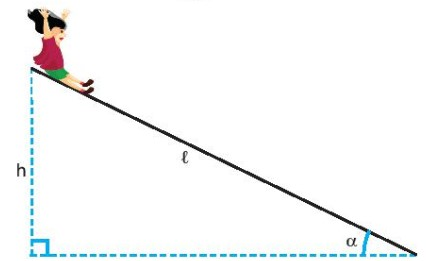
\includegraphics[scale=0.8]{../figs/VN10-2022-PH-TP030-1.jpg}
		\end{center}
		
		Độ cao của đỉnh cầu trượt so với mặt đất:
		
		$$ h = l\sin \alpha \approx \SI{2,57}{m}.$$
		
		Do có ma sát khi trượt, một phần thế năng của em bé được chuyển hóa thành động năng, một phần thắng công cản $A$ của lực ma sát:
		
		$$mgh - \dfrac{1}{2}mv^2 = A \Rightarrow A \approx \SI{411,6}{J}.$$
		
		Độ lớn của lực ma sát
		
		$$F_\text{ms} = \dfrac{A}{l} \approx \SI{102,9}{N}.$$
		
		Năng lượng toàn phần = thế năng của em bé ở đỉnh cầu trượt:
		
		$$W = mgh = \SI{514}{J}.$$
		
		Năng lượng hao phí bằng độ lớn công của lực ma sát. 
		
		Năng lượng có ích
		
		$$W_\text{ci} = W - A = \SI{102,4}{J}.$$
		
		Hiệu suất của quá trình biến đổi thế năng thành động năng:
		
		$$H = \dfrac{W_\text{ci}}{W} \cdot 100\% \approx 20\%.$$
	}
	
\end{enumerate}